\chapter{Mengenal Kecerdasan Buatan dan Scikit-Learn}
Buku umum yang digunakan adalah \cite{russell2016artificial} dan  
untuk sebelum UTS menggunakan buku \textit{Python Artificial Intelligence Projects for Beginners}\cite{eckroth2018python}.
Dengan praktek menggunakan python 3 dan editor anaconda dan library python scikit-learn.
Tujuan pembelajaran pada pertemuan pertama antara lain:
\begin{enumerate}
\item
Mengerti definisi kecerdasan buatan, sejarah kecerdasan buatan, perkembangan dan penggunaan di perusahaan
\item
Memahami cara instalasi dan pemakaian sci-kit learn
\item
Memahami cara penggunaan variabel explorer di spyder
\end{enumerate}
Tugas dengan cara dikumpulkan dengan pull request ke github dengan menggunakan latex pada repo yang dibuat oleh asisten riset.

\section{Teori}
Praktek teori penunjang yang dikerjakan :
\begin{enumerate}
\item
Buat Resume Definisi, Sejarah dan perkembangan Kecerdasan Buatan, dengan bahasa yang mudah dipahami dan dimengerti. Buatan sendiri bebas plagiat[hari ke 1](10)
\item
Buat Resume mengenai definisi supervised learning, klasifikasi, regresi dan unsupervised learning. Data set, training set dan testing set.[hari ke 1](10)
\end{enumerate}

\section{Instalasi}
Membuka https://scikit-learn.org/stable/tutorial/basic/tutorial.html. Dengan menggunakan bahasa yang mudah dimengerti dan bebas plagiat. 
Dan wajib skrinsut dari komputer sendiri.
\begin{enumerate}
\item
Instalasi library scikit dari anaconda, mencoba kompilasi dan uji coba ambil contoh kode dan lihat variabel explorer[hari ke 1](10)
\item
Mencoba Loading an example dataset, menjelaskan maksud dari tulisan tersebut dan mengartikan per baris[hari ke 1](10)
\item
Mencoba Learning and predicting, menjelaskan maksud dari tulisan tersebut dan mengartikan per baris[hari ke 2](10)
\item
mencoba Model persistence, menjelaskan maksud dari tulisan tersebut dan mengartikan per baris[hari ke 2](10)
\item 
Mencoba Conventions, menjelaskan maksud dari tulisan tersebut dan mengartikan per baris[hari ke 2](10)
\end{enumerate}


\section{Penanganan Error}
Dari percobaan yang dilakukan di atas, apabila mendapatkan error maka:

\begin{enumerate}
	\item
	skrinsut error[hari ke 2](10)
	\item
Tuliskan kode eror dan jenis errornya [hari ke 2](10)
	\item
Solusi pemecahan masalah error tersebut[hari ke 2](10)

\end{enumerate}


\section{andi muh aslam/1164064}
\subsection{sejarah dan perkembangan kecerdasan buatan}
\begin{enumerate}
\item didefinisikan  kecerdasan yang ditunjukkan oleh suatu entitas buatan. Umumnya dianggap komputer. Kecerdasan Buatan (Artificial Intelligence atau AI) didefinisikan sebagai kecerdasan yang ditunjukan oleh suatu entitas buatan. Sistem seperti ini umumnnya dianggao kemputer. Kecerdasan dimasukkan ke dalam mesin (komputer) agar dapat melakukan pekerjaan seperti yang dapat dilakukan manusia. Kecerdasan Buatan (Artificial Intelligence atau AI) didefinikasikan sebagai kecerdasan yang ditinjukkan oleh suatu entitas buatan. Sistem seperti ini umumnya di anggap komputer. Kecerdasan diciptakan dan dimasukkan melakukan pekerjaan seperti yang dapat dilakukan manusia. 
\item Sejarah dan perkembangan kecerdasan buatan terjadi pada musim panas tahun 1956 tercatat adanya seminar mengenai AI di Darmouth College. Seminar pada waktu itu dihadiri oleh sejumlah pakar komputer dan membahas potensi komputer dalam meniru 
kepandaian manusia. Akan tetapi perkembangan yang sering terjadi semenjak diciptakannya LISP, yaitu bahasa kecerdasan buatan yang dibuat tahun 1960 oleh John McCarthy. Istilah pada kecerdasan buatan atau Artificial Intelligence diambil dari Marvin Minsky dari MIT. Dia menulis karya ilmiah berjudul Step towards Artificial Intelligence,The Institute of radio Engineers Proceedings 49, January 1961\cite{nasution2012implementasi}.
\item Supervised learning merupakan sebuah pendekatan dimana sudah terdapat data yang dilatih, dan terdapat variable yang ditargetkan sehingga tujuan dari pendekatan ini adalah mengkelompokan suatu data ke data yang sudah ada. Sedangkan unsupervised 
learning tidak memiliki data latih, sehingga dari data yang ada, kita mengelompokan data tersebut menjadi 2 bagian atau 3 bagian dan seterusnya.
\item Klasifikasi adalah salah satu topik utama dalam data mining atau machine learning. Klasifikasi yaitu suatu pengelompokan data dimana data yang digunakan tersebut mempunyai kelas label atau target.
\item Regresi adalah Supervised learning tidak hanya mempelajari classifier, tetapi juga mempelajari fungsi yang dapat memprediksi suatu nilai numerik. Contoh, ketika diberi foto seseorang, kita ingin memprediksi umur, tinggi, dan berat orang yang ada pada foto tersebut.
\item Data set adalah cabang aplikasi dari Artificial Intelligence/Kecerdasan Buatan yang fokus pada pengembangan sebuah sistem yang mampu belajar sendiri tanpa harus berulang kali di program oleh manusia.
\item Training set yaitu jika pasangan objek, dan kelas yang menunjuk pada objek tersebut adalah suatu contoh yang telah diberi label akan menghasilkan suatu algoritma pembelajaran.
\subitem Testing set digunakan untuk mengukur sejauh mana classifier berhasil melakukan klasifikasi dengan benar\cite{darujati2012pemanfaatan}.
\end{enumerate}


\section{Instalasi}
\subsection{instalasi Library Scikit dari Anaconda}
\begin{enumerate}
\item Download aplikasi Anaconda terlebih dahulu
\begin{figure} [ht]
\centering
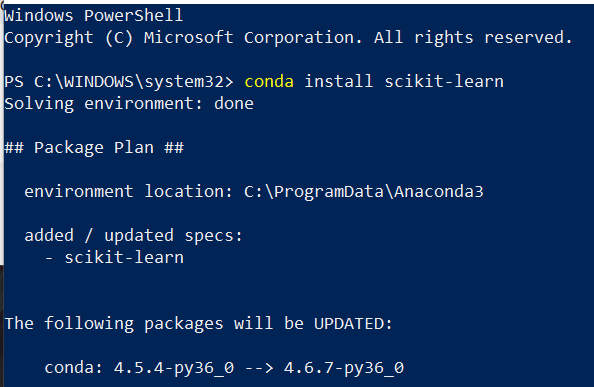
\includegraphics[scale=1] {figures/1.png}
\caption{Langkah 1 instalasi anaconda..}
\end{figure}

\item Proceed install anaconda 
\begin{figure} [ht]
\centering
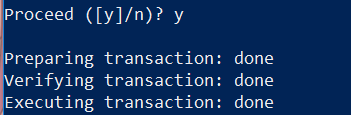
\includegraphics[scale=1] {figures/2.png}
\caption{Langkah 2 instalasi anaconda.}
\end{figure}

\item install scikit-learn
\begin{figure} [ht]
\centering 
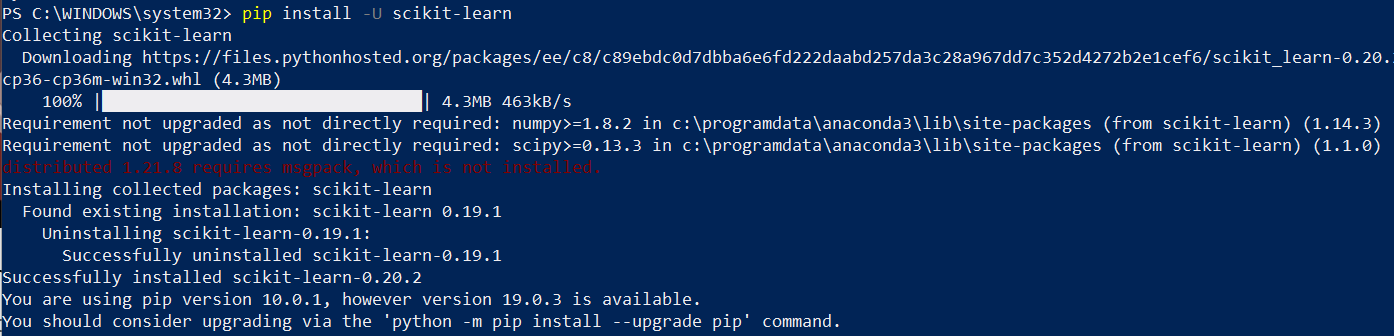
\includegraphics[scale=1] {figures/4.png}
\caption{Langkah 3 instalasi anaconda. }
\end{figure}

\item perintah print
\begin{figure} [ht]
\centering 
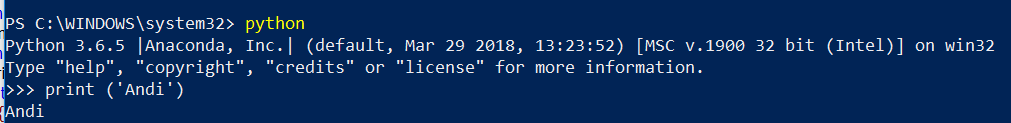
\includegraphics[scale=1] {figures/5.png}
\caption{Langkah 4 instalasi anaconda. }
\end{figure}
\end{enumerate}

\subsubsection{Mencoba Loading an example dataset}
\begin{enumerate}
\item Masuk Pyhton terlebih dahulu
\begin{figure} [ht]
\centering 
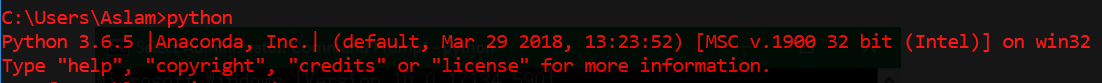
\includegraphics[scale=1] {figures/6.png}
\caption{Langkah 1 dataset. }
\end{figure}

\item from sklearn import datasets(pada baris ini merupakan sebuah perintah untuk mengimport sebuah datasets dari file sklearn).
\begin{figure} [ht]
\centering 
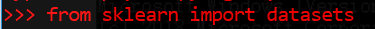
\includegraphics[scale=1] {figures/7.png}
\caption{Langkah 2 dataset. }
\end{figure}

\item iris \= datasets.load\_iris()(pada baris kedua ini dimana iris merupakan suatu variable yang berfungsi untuk mengambil data pada datasets dengan perintah .load\_iris).
\begin{figure} [ht]
\centering 

\includegraphics[scale=1] {figures/8.png}
\caption{Langkah 3 dataset. }
\end{figure}

\item digits \= datasets.load\_digits()(pada baris ketiga ini dimana digits merupakan suatu variable yang berfungsi untuk mengambil data pada datasets dengan perintah .load\_digits)
\begin{figure} [ht]
\centering 
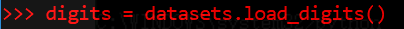
\includegraphics[scale=1] {figures/9.png}
\caption{Langkah 4 dataset. }
\end{figure}

\item print(digits.data)(pada baris keempat ini merupakan perintah yang berfungsi untuk memanggil atau menampilkan variable digits.data)
\begin{figure} [ht]
\centering 
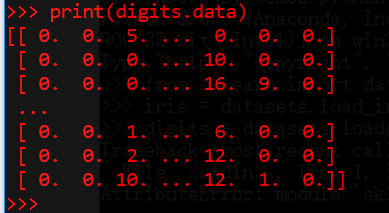
\includegraphics[scale=1] {figures/10.png}
\caption{Langkah 5 dataset. }
\end{figure}
<<<<<<< HEAD

\section{Aip Suprapto Munari/1164063}
\subsection{Teori}
\begin{enumerate}
\item Definisi, sejarah, dan perkembangan kecerdasan buatan.
\subitem Definisi kecerdasan buatan adalah ilmu pengetahuan yang dapat membuat komputer untuk meniru kecerdasan manusia yang berhubungan dengan penangkapan, pemodelan, dan penyimpanan kecerdasan manusia dalam sebuah sistem teknologi. Contohnya yaitu melakukan analisa penalaran untuk mengambil suatu kesimpulan atau penerjemahan atau keputusan dari satu bahasa satu ke bahasa lain.
\subitem Sejarah dan perkembangan kecerdasan buatan terjadi pada musim panas tahun 1956 tercatat adanya seminar mengenai AI di Darmouth College. Seminar pada waktu itu dihadiri oleh sejumlah pakar komputer dan membahas potensi komputer dalam meniru kepandaian manusia. Akan tetapi perkembangan yang sering terjadi semenjak diciptakannya LISP, yaitu bahasa kecerdasan buatan yang dibuat tahun 1960 oleh John McCarthy. Istilah pada kecerdasan buatan atau Artificial Intelligence diambil dari Marvin Minsky dari MIT. Dia menulis karya ilmiah berjudul Step towards Artificial Intelligence, The Institute of radio Engineers Proceedings 49, January 1961\cite{baraja2008kecerdasan}. 
\item  Definisi supervised learning, klasifikasi, regresi, dan unsupervised learning. Data set, training set dan testing set. 
\subitem Supervised learning merupakan sebuah pendekatan dimana sudah terdapat data yang dilatih, dan terdapat variable yang ditargetkan sehingga tujuan dari pendekatan ini adalah mengkelompokan suatu data ke data yang sudah ada. Sedangkan unsupervised learning tidak memiliki data latih, sehingga dari data yang ada, kita mengelompokan data tersebut menjadi 2 bagian atau 3 bagian dan seterusnya.
\subitem Klasifikasi merupakan salah satu topik utama dalam data mining atau machine learning. Klasifikasi yaitu suatu pengelompokan data dimana data tersebut digunakan untuk mempunyai kelas label atau target.
\subitem Regresi adalah Supervised learning tidak hanya mempelajari classifier, tetapi juga mempelajari fungsi yang dapat memprediksi suatu nilai numerik. Contoh, ketika diberi foto seseorang, kita ingin memprediksi umur, tinggi, dan berat orang yang ada pada foto tersebut.
\subitem Data set adalah cabang aplikasi dari Artificial Intelligence/Kecerdasan Buatan yang fokus pada pengembangan sebuah sistem yang mampu belajar sendiri tanpa harus berulang kali di program oleh manusia.
\subitem Training set yaitu jika pasangan objek, dan kelas yang menunjuk pada objek tersebut adalah suatu contoh yang telah diberi label akan menghasilkan suatu algoritma pembelajaran.
\subitem Testing set digunakan untuk mengukur sejauh mana classifier berhasil melakukan klasifikasi dengan benar\cite{zhu2009introduction}.
\end{enumerate}
\subsection{Instalasi}
\subsubsection{Instalasi Library Scikit dari Anaconda}
\begin{enumerate}
\item Download aplikasi Anaconda terlebih dahulu. Lihat pada gambar 1.1
\item Install aplikasi Anaconda yang sudah di download tadi. Lihat pada gambar 1.2
\item Centang Keduanya lalu tekan tombol install. Lihat pada gambar 1.3
\item Setelah itu tunggu sampai proses instalasi selesai lalu jika sudah tekan tombol finish. Lihat pada gambar 1.4
\item Lalu buka command prompt anda dan tuliskan perintah berikut ini untuk mengecek apakah aplikasinya sudah terinstall. Lihat pada gambar 1.5
\item Kemudian ketikkan perinta pip install -U scikit-learn seperti gambar berikut. Lihat pada gambar 1.6
\item Lalu jika sudah  ketikkan juga perintah conda install scikit-learn. Lihat pada gambar 1.7
\item dan setelah itu pilih y. Lihat pada gambar 1.8
\item Hasil version yang diinstall. Lihat pada gambar 1.9
\end{enumerate}
\subsubsection{Mencoba Loading an example Dataset}
\begin{itemize}
\item from sklearn import datasets(pada baris ini merupakan sebuah perintah untuk mengimport class datasets dari packaged sklearn).
\item iris = datasets.load\_iris()(pada baris kedua ini dimana iris merupakan suatu estimator/parameter yang berfungsi untuk mengambil data pada item datasets.load\_iris).
\item digits = datasets.load\_digits()(pada baris ketiga ini dimana digits merupakan suatu estimator/parameter yang berfungsi untuk mengambil data pada item datasets.load\_digits).
\item print(digits.data)(pada baris keempat ini merupakan perintah yang berfungsi untuk menampilkan estimator/parameter yang dipanggil pada item digits.data dan menampilkan outputannya) Lihat gambar 1.10.
\item digits.target(barisan ini untuk mengambil target pada estimator/parameter digits dan menampilkan outputannya) Lihat gambar 1.11.
\item digits.images[0](barisan ini untuk mengambil images[0] pada estimator/parameter digits dan menampilkan outputannyal) Lihat gambar 1.12.
\end{itemize}
=======
\end{enumerate}

>>>>>>> 78cdb6514db9716f252ef2024a7df6097aace611
\subsubsection{Learning and Predicting}
\begin{itemize}
\item from sklearn import svm(pada baris ini merupakan sebuah perintah untuk mengimport class svm dari packaged sklearn).
\item clf = svm.SVC(gamma=0.001, C=100.)(pada baris kedua ini clf sebagai estimator/parameter, svm.SVC sebagai class, gamma sebagai parameter untuk menetapkan nilai secara manual)
\item clf.fit(digits.data[:-1], digits.target[:-1])(pada baris ketiga ini clf sebagai estimator/parameter, fit sebagai metode, digits.data sebagai item, [:-1] sebagai syntax pythonnya dan menampilkan outputannya) Lihat gambar 1.13.
\item clf.predict(digits.data[-1:])
\end{itemize}
<<<<<<< HEAD
\subsection{Mencoba Model Persistance, menjelaskan maksud dari tulisan tersebut dan mengartikan per baris}
\begin{enumerate}
\item
Pada Python Shell ketikan "from sklearn import svm" artinya akan mengimport sebuah Support Vector Machine(SVM) yang merupakan algoritma classification yang akan diambil dari Scikit-Learn.
\item
Kemudian, lanjutkan dengan "from sklearn import datasets" yang artinya akan mengambil package datasets dari Scikit-Learn.
\item
ketikan, clf = svm.SVC(gamma='scale') berfungsi untuk mendeklarasikan suatu value yang bernama clf yang berisi gamma. Parameter gamma menentukan seberapa jauh pengaruh dari satu contoh training.
\item
Ketikan, X, y = iris.data, iris.target, artinya X sebagai data iris, dan y merupakan larik target.
\item
Ketikan, clf.fit(X, y) berfungsi untuk melakukan pengujian classifier. hasilnya seperti ini
\begin{figure}
	\begin{center}
   	 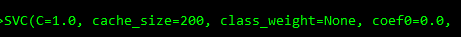
\includegraphics[scale=1]{figures/aip7.png}
   	 \caption{Hasil Pengujian Classifier}	
	\end{center}
\end{figure}
\item
\begin{figure}
	\begin{center}
   	 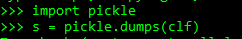
\includegraphics[scale=1]{figures/aip8.png}
   	 \caption{Hasil Pengujian Classifier}	
	\end{center}
\end{figure}
Dari gambar diatas dapat dijelaskan bahwa akan mengimport Pickle dari Python. Pickle digunakan untuk serialisasi dan de-serialisasi struktur objek Python. Objek apa pun dengan Python dapat di-Pickle sehingga dapat disimpan di disk. kemudian menyimpan data objek ke file CLF sebelumnya dengan menggunakan function pickle.dumps(clf).
\item
Setelah mengetikan fungsi fungsi diatas, selanjutnya ketikan "clf2 = pickle.loads(s)" yang artinya pickle.loads digunakan untuk memuat data pickle dari string byte. "S" dalam loads mengacu pada fakta bahwa dalam Python 2, data dimuat dari string.
\begin{figure}
	\begin{center}
   	 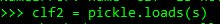
\includegraphics[scale=1]{figures/aip9.png}
   	 \caption{Pickle Pada Python}	
	\end{center}
\end{figure}
\item
\begin{figure}
	\begin{center}
   	 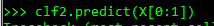
\includegraphics[scale=1]{figures/aip10.png}
   	 \caption{Pengujian Classifier Pickle}	
	\end{center}
\end{figure}
Pada gambar diatas dilakukan pengujian nilai baru dengan menggunakan "cf2.predict(X[0:1])" dengan target asumsinya (0,1) hasilnya berbentuk array.
\item
Dalam kasus khusus scikit-learn, mungkin lebih menarik untuk menggunakan joblib (dump dan load) untuk menggantikan Pickle, yang lebih efisien pada data besar tetapi hanya bisa di Pickle ke disk dan tidak ke string. untuk menggunakan Joblib pertama ketikan "from joblib import dump , load" yang artinya akan Merekonstruksi objek Python dari file yang sudah ada.\\

dump(clf, 'filename.joblib') akan merekontruksi file CLF yang tadi sudah dideklarasikan.\\
clf = load('filename.joblib') untuk mereload model yang sudah di Pickle\\
\begin{figure}
	\begin{center}
   	 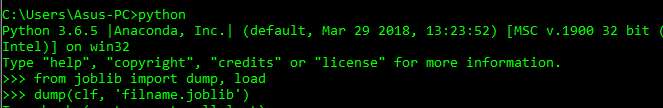
\includegraphics[scale=1]{figures/aip11.png}
   	 \caption{Penggunaan Joblib}	
	\end{center}
\end{figure}
\end{enumerate}

\subsection{Mencoba Conventions, menjelaskan maksud dari tulisan tersebut dan mengartikan per baris}
\begin{enumerate}
\item
Import numpy as np, digunakan untuk mengimport Numpy sebagai np.\\
From sklearn import randomprojection artinya modul yang mengimplementasikan cara sederhana dan efisien secara komputasi untuk mengurangi dimensi data dengan memperdagangkan sejumlah akurasi yang terkendali (sebagai varian tambahan) untuk waktu pemrosesan yang lebih cepat dan ukuran model yang lebih kecil.
\begin{figure}
	\begin{center}
   	 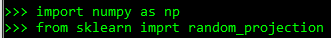
\includegraphics[scale=1]{figures/aip12.png}
   	 \caption{Deklarasi Numpy}	
	\end{center}
\end{figure}
\item
\begin{figure}
	\begin{center}
   	 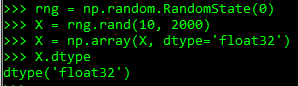
\includegraphics[scale=1]{figures/aip13.png}
   	 \caption{Contoh Type Casting}	
	\end{center}
\end{figure}
Pada gambar diatas dapat dijelaskan bahwa :\\
rng = np.random.RandomState(0), digunakan untuk menginisialisasikan random number generator.\\
X = rng.rand(10, 2000) artinya akan merandom value antara 10 sampai 2000.\\
X = np.array(X, dtype='float32') Array numpy terdiri dari buffer memori "mentah" yang diartikan sebagai array melalui "views". Anda dapat menganggap semua array numpy sebagai tampilan. Mendeklarasikan X sebagai float32.
\item
Dalam contoh ini, X adalah float32, yang dilemparkan ke float64 oleh fittransform (X).
\begin{figure}
	\begin{center}
   	 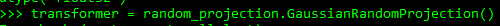
\includegraphics[scale=1]{figures/aip14.png}
   	 \caption{Menggunakan FitTransform}
	\end{center}
\end{figure}
\item
Target regresi dilemparkan ke float64 dan target klasifikasi dipertahankan.

list(clf.predict(irisdata[:3])), akan memprediksi 3 data dari iris.\\
clf.fit irisdata, iristargetnames[iristarget] menguji classifier dengan ada targetnya yaitu irisnya sendiri.\\
list(clf.predict(irisdata[:3])), setelah diuji maka akan muncul datanya seperti dibawah ini\\
\begin{figure}
	\begin{center}
   	 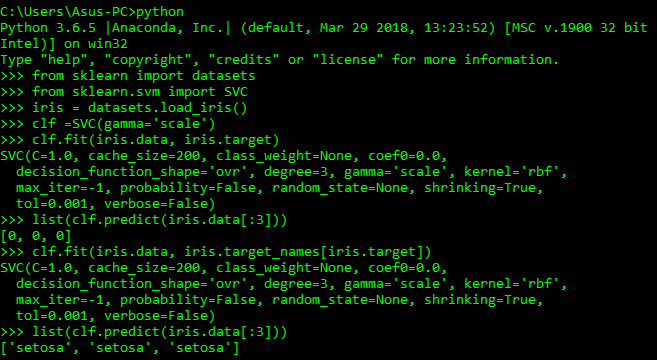
\includegraphics[scale=1]{figures/aip15.png}
   	 \caption{Regresi Yang Dilempar}
	\end{center}
\end{figure}
Di sini, prediksi pertama () mengembalikan array integer, karena iristarget (array integer)yang digunakan sesuai. Prediksi kedua () mengembalikan array string, karena iristargetnames cocok.
\item
Refitting dan Memperbaharui Parameter

y = rngbinomial(1, 0.5, 100) , random value dengan angka binomial atau suku dua untuk y \\
clfsetparams(kernel='linear')fit(X, y) mengubahn kernel default menjadi linear \\
clfsetparams(kernel='rbf', gamma='scale')fit(X, y)  Di sini, kernel default rbf pertama kali diubah menjadi linear melalui\\ SVCsetparams () setelah estimator dibuat, dan diubah kembali ke rbf untuk mereparasi estimator dan membuat prediksi kedua.
\begin{figure}
	\begin{center}
   	 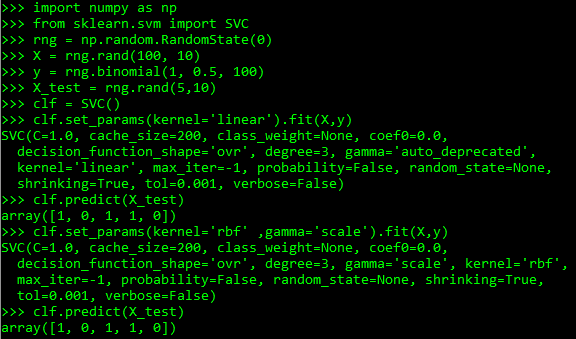
\includegraphics[scale=1]{figures/aip16.png}
   	 \caption{Refitting dan Memperbaharui Parameter}
	\end{center}
\end{figure}
\item
MultiClass VS MultiLabel Classifier \\
from sklearn.multiclass import OneVsRestClassifier ,adalah  ketika kita ingin melakukan klasifikasi multiclass atau multilabel dan baik unutk menggunakan OneVsRestClassifier per kelas. Untuk setiap classifier, kelas tersebut dipasang terhadap semua kelas lainnya. (Ini cukup jelas dan itu berarti bahwa masalah klasifikasi multiclass / multilabel dipecah menjadi beberapa masalah klasifikasi biner).\\
from sklearn.preprocessing import LabelBinarizer ,adalah kelas utilitas untuk membantu membuat matriks indikator label dari daftar label multi-kelas\\
Dalam gambar dibawah, classifier cocok pada array 1d label multiclass dan oleh karena itu metode predict () memberikan prediksi multiclass yang sesuai.
\begin{figure}
	\begin{center}
   	 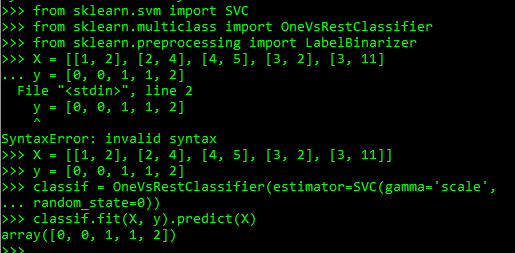
\includegraphics[scale=1]{figures/aip17.png}
   	 \caption{MultiClass Classifier}
	\end{center}
\end{figure}
\item
Di sini, classifier cocok () pada representasi label biner 2d dari y, menggunakan LabelBinarizer. Dalam hal ini predict () mengembalikan array 2d yang mewakili prediksi multilabel yang sesuai.
\begin{figure}
	\begin{center}
   	 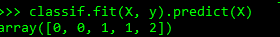
\includegraphics[scale=1]{figures/aip18.png}
   	 \caption{MultiClass Classifier biner 2D}
	\end{center}
\end{figure}
\item
from sklearn.preprocessing import MultiLabelBinarizer , artinya Transformasi antara iterable dari iterables dan format multilabel.\\
Dalam hal ini, penggolongnya sesuai pada setiap instance yang diberi beberapa label. MultiLabelBinarizer digunakan untuk membuat binarize array 2d dari multilabel agar sesuai. Hasilnya, predict () mengembalikan array 2d dengan beberapa label yang diprediksi untuk setiap instance.
\begin{figure}
	\begin{center}
   	 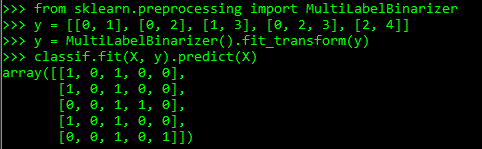
\includegraphics[scale=1]{figures/aip19.png}
   	 \caption{MultiLabel Classifier}
	\end{center}
\end{figure}
\end{enumerate}


\section{Penanganan Error}
HARI KEDUA
\begin{enumerate}
	\item
	Berikut ini merupakan eror yang ditemui pada saat melakukan percobaan skrip.
\begin{figure}
	\begin{center}
   	 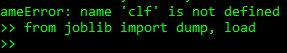
\includegraphics[scale=1]{figures/eror2.png}
   	 \caption{Eror Import}
	\end{center}
\end{figure}
	\item
Pada gambar eror diatas, kode erornya adalah "ImportError: No Module Named" artinya mengalami masalah saat mengimpor modul yang ditentukan.
	\item
Solusinya bisa dilakukan seperti berikut :\\
eror diats terjadi dikarenakan Library Joblib belum terinstal pada PC. Maka dari itu sekarang kita harus menginstalnya dulu.
	\item
Buka CMD, kemudian ketikan "pip install joblib" tunggu sampai instalasi berhasil seperti gambar berikut.
\begin{figure}
	\begin{center}
   	 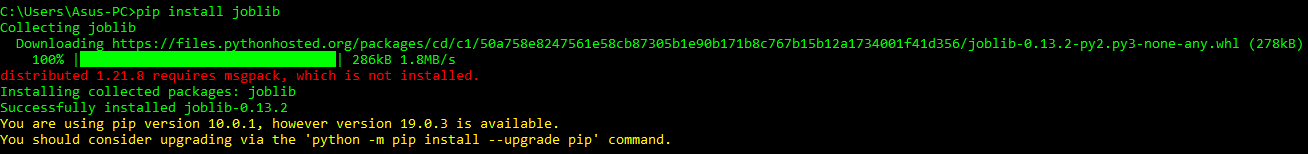
\includegraphics[scale=1]{figures/solusi2.png}
   	 \caption{Instal Library Joblib}
	\end{center}
\end{figure}
	\item
Apabila sudah terinstall, dapat dilakukan lagi import library joblib, maka akan berhasil seperti dibawah berikut
\begin{figure}
	\begin{center}
   	 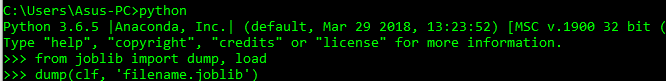
\includegraphics[scale=1]{figures/solusi2_1.png}
   	 \caption{Berhasil Import Library Joblib}
	\end{center}
\end{figure}
\end{enumerate}

\begin{figure}[ht]\centerline{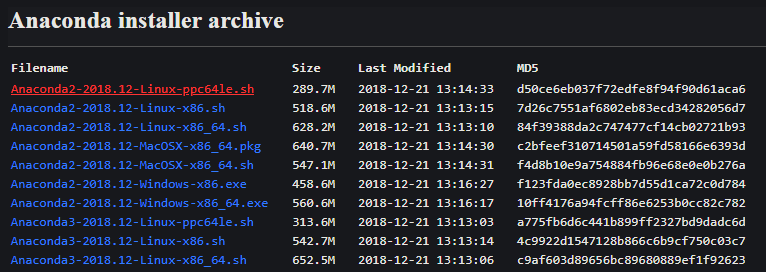
\includegraphics[width=1\textwidth]{figures/a1.PNG}}\caption{Download Anaconda.}\end{figure}
\begin{figure}[ht]\centerline{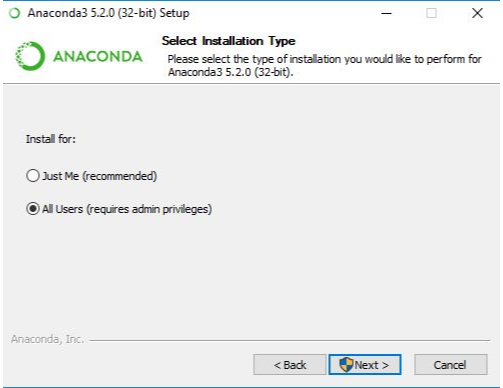
\includegraphics[width=0.75\textwidth]{figures/a2.PNG}}\caption{Langkah pertama instalasi anaconda.}\end{figure}
\begin{figure}[ht]\centerline{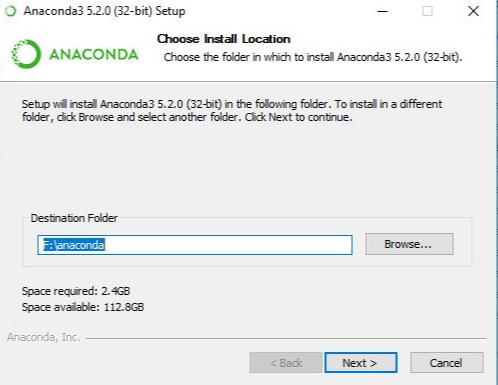
\includegraphics[width=0.75\textwidth]{figures/a3.PNG}}\caption{Langkah kedua instalasi anaconda.}\end{figure}
\begin{figure}[ht]\centerline{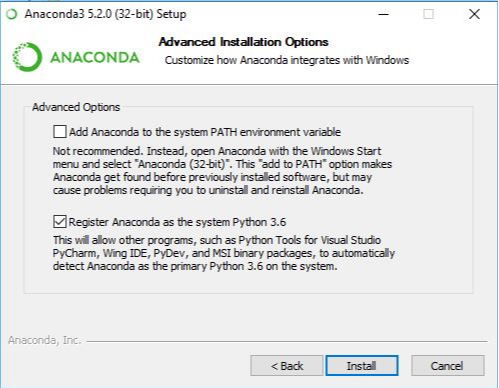
\includegraphics[width=0.75\textwidth]{figures/a4.PNG}}\caption{Langkah ketiga instalasi anaconda.}\end{figure}
\begin{figure}[ht]\centerline{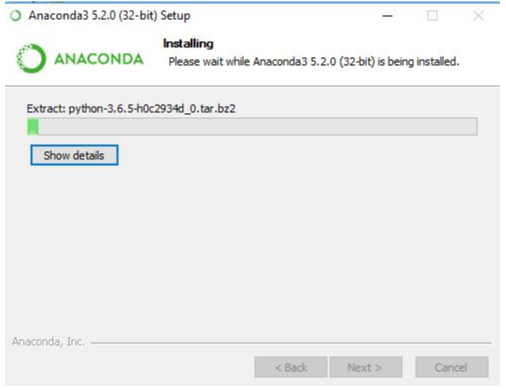
\includegraphics[width=0.75\textwidth]{figures/a5.PNG}}\caption{Langkah terakhir instalasi anaconda.}\end{figure}
\begin{figure}[ht]\centerline{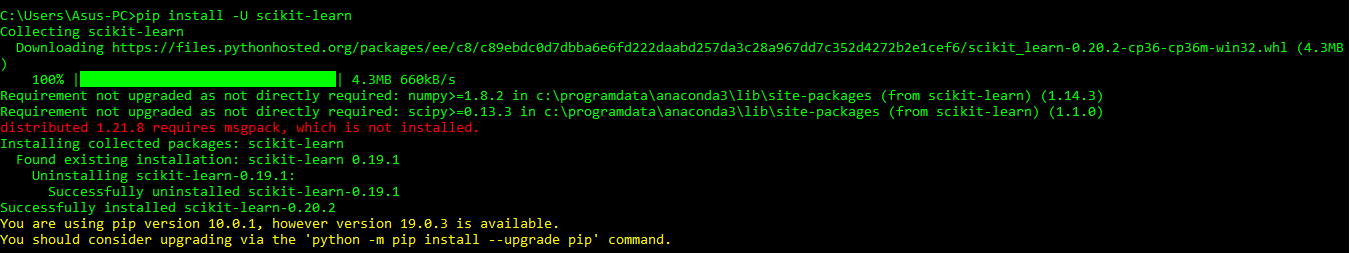
\includegraphics[width=0.75\textwidth]{figures/a6.PNG}}\caption{Langkah pertama instalasi scikit pada CMD.}\end{figure}
\begin{figure}[ht]\centerline{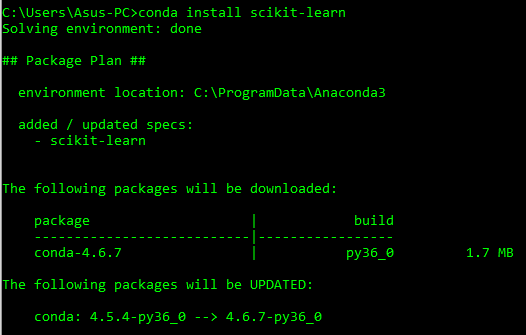
\includegraphics[width=0.75\textwidth]{figures/a7.PNG}}\caption{Langkah ketiga instalasi conda scikit pada CMD.}\end{figure}
\begin{figure}[ht]\centerline{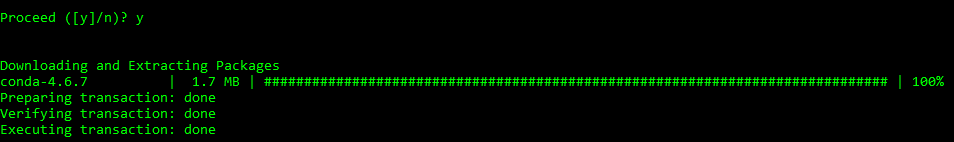
\includegraphics[width=0.75\textwidth]{figures/a8.PNG}}\caption{Langkah kedua pilih y.}\end{figure}
\begin{figure}[ht]\centerline{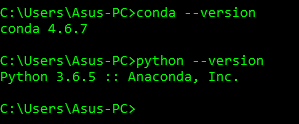
\includegraphics[width=0.75\textwidth]{figures/a9.PNG}}\caption{Langkah cek version yang diinstall.}\end{figure}
\begin{figure}[ht]\centerline{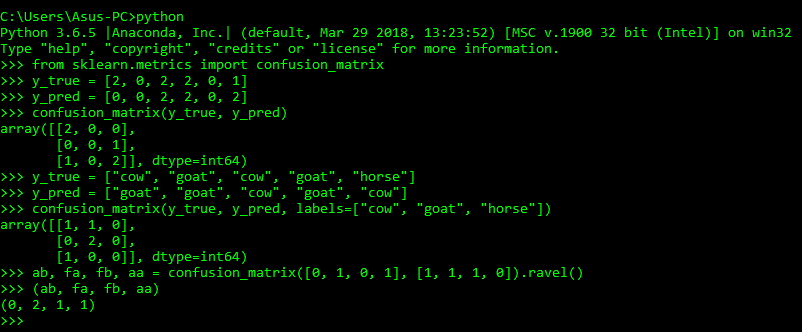
\includegraphics[width=0.75\textwidth]{figures/a10.PNG}}\caption{Hasil Tampilan 1.}\end{figure}
\begin{figure}[ht]\centerline{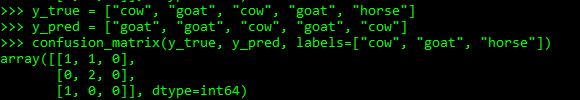
\includegraphics[width=0.75\textwidth]{figures/a11.PNG}}\caption{Hasil Tampilan 2.}\end{figure}
\begin{figure}[ht]\centerline{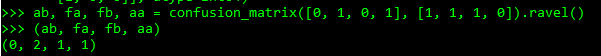
\includegraphics[width=0.75\textwidth]{figures/a12.PNG}}\caption{Hasil Tampilan 3.}\end{figure}
=======

\subsubsection{Model Presistence}
\begin{itemize}
\item from sklearn import svm(pada baris ini merupakan sebuah perintah untuk mengimport class svm dari packaged sklearn).
\item from sklearn import datasets(pada baris ini merupakan sebuah perintah untuk mengimport class datasets dari packaged sklearn).
\item\begin{verbatim} clf = svm.SVC(gamma='scale')\end{verbatim}(pada baris ketga ini clf sebagai estimator/parameter, svm.SVC sebagai class, gamma sebagai parameter untuk menetapkan nilai secara manual dengan nilai scale).
\item\begin{verbatim} iris = datasets.load_iris()\end{verbatim}(pada baris keempat ini iris sebagai estimator/parameter, datasets.load\_iris() sebagai item dari suatu nilai).
\item\begin{verbatim} X, y = iris.data, iris.target\end{verbatim}(pada baris kelima ini X, y sebagai estimator/parameter, iris.data, iris.target sebagai item dari 2 nilai yang ada).
\item\begin{verbatim} clf.fit(X, y)\end{verbatim}(pada baris keenam ini clf sebagai estimator/parameter dengan menggunakan metode fit untuk memanggil estimator X, y dengan outputannya) 
\item\begin{verbatim} import pickle\end{verbatim}(pickle merupakaan sebuah class yang di import).
\item\begin{verbatim} s = pickle.dumps(clf)\end{verbatim}(pada baris ini s sebagai estimator/parameter dengan pickle.dumps merupakan suatu nilai/item dari estimator/parameter clf)
\item\begin{verbatim} clf2 = pickle.loads(s)\end{verbatim}(pada baris ini clf2 sebagai estimator/parameter, pickle.loads sebagai suatu item, dan s sebagai estimator/parameter yang dipanggil) 
\item\begin{verbatim} clf2.predict(X[0:1])\end{verbatim}(pada baris ini clf2.predict sebagai suatu item dengan menggunakan metode predict untuk menentukkan suatu nilai dari (X[0:1])) 
\item\begin{verbatim} y[0]\end{verbatim}(pada estimator/parameter y berapapun angka yang diganti nilainya akan selalu konstan yaitu 0)
\item\begin{verbatim} from joblib import dump, load\end{verbatim}(pada baris berikut ini merupakan sebuah perintah untuk mengimport class dump, load dari packaged joblib).
\item\begin{verbatim} dump(clf, 'filename.joblib')\end{verbatim}(pada baris berikutnya dump di sini sebagai class yang didalamnya terdapat nilai dari suatu item clf dan data joblib).
\item\begin{verbatim} clf = load('filename.joblib')\end{verbatim}(pada baris terakhir clf sebagai estimato/parameter dengan suatu nilai load berfungsi untuk mengulang data sebelumnya)
\item dari ketiga baris akhir tersebut jika di jalankan aau dituliskan perintah seperti itu maka akan menampilkan tampilan eror 
\end{itemize}

\subsubsection{Conventions}
\begin{enumerate}
\item Type Casting
\begin{itemize}
\item\begin{verbatim} from sklearn import svm\end{verbatim}(pada baris ini merupakan sebuah perintah untuk mengimport class svm dari packaged sklearn).
\item\begin{verbatim} from sklearn import random_projection\end{verbatim}(pada baris ini merupakan sebuah perintah untuk mengimport class random\_projection dari packaged sklearn).
\item\begin{verbatim} rng = np.random.RandomState(0)\end{verbatim}(rng sebagai estimator/parameter dengan nilai suatu itemnya yaitu np.random.RandomState(0)).
\item\begin{verbatim} X = rng.rand(10, 2000)\end{verbatim}(X sebagai estimator/parameter dengan nilai item rng.rand).
\item\begin{verbatim} X = np.array(X, dtype='float32')\end{verbatim}(X sebagai estimator/parameter dengan nilai item np.array).
\item\begin{verbatim} X.dtype\end{verbatim}(X.dtype sebagai item pemanggil) 
\item\begin{verbatim} transformer = random_projection.GaussianRandomProjection()\end{verbatim}(transformer sebagai estimator/parameter dengan memanggil class random\_projection).
\item\begin{verbatim} X_new = transformer.fit_transform(X)\end{verbatim}(X\_new di sini sebagai estomator/parameter dan menggunakan metode fit)
\item\begin{verbatim} X_new.dtype\end{verbatim}(X\_new.dtype sebagai item) 
\item\begin{verbatim} from sklearn import datasets\end{verbatim}(pada baris ini merupakan sebuah perintah untuk mengimport class datasets dari packaged sklearn).
\item\begin{verbatim} from sklearn.svm import SVC\end{verbatim}(pada baris ini merupakan sebuah perintah untuk mengimport class SVC dari packaged sklearn.svm).
\item\begin{verbatim} iris = datasets.load_iris()\end{verbatim}(iris sebagai estimator/parameter dengan item datasets.load\_iris()).
\item\begin{verbatim} clf = SVC(gamma='scale')\end{verbatim}(clf sebagai estimator/parameter dengan nilai class SVC pada parameter gamma sebagai set penilaian).
\item\begin{verbatim} clf.fit(iris.data, iris.target)\end{verbatim}(estimator/parameter clf menggunakan metode fit dengan itemnya) 
\item\begin{verbatim} list(clf.predict(iris.data[:3]))\end{verbatim}(menambahkan item list dengan metode predict) 
\item\begin{verbatim} clf.fit(iris.data, iris.target_names[iris.target])\end{verbatim}(estimator/parameter clf menggunakan metode fit dengan itemnya)
\item\begin{verbatim} list(clf.predict(iris.data[:3]))(menambahkan item list dengan metode predict\end{verbatim} 
\end{itemize}
\item Refitting and Updating Parameters
\begin{itemize}
\item\begin{verbatim} import numpy as np\end{verbatim}(pada baris ini merupakan sebuah perintah untuk mengimport class svm dari np).
\item\begin{verbatim} from sklearn.svm import SVC\end{verbatim}(pada baris ini merupakan sebuah perintah untuk mengimport class SVC dari packaged sklearn.svm).
\item\begin{verbatim} rng = np.random.RandomState(0)\end{verbatim}(rng sebagai estimator/parameter dengan nilai suatu itemnya yaitu np.random.RandomState(0)).
\item\begin{verbatim} X = rng.rand(100, 10)\end{verbatim}(X sebagai estimator/parameter dengan nilai item rng.rand).
\item\begin{verbatim} y = rng.binomial(1, 0.5, 100)\end{verbatim}(y sebagai estimator/parameter dengan nilai item rng.binomial).
\item\begin{verbatim} X_test = rng.rand(5, 10)\end{verbatim}(X\_test sebagai estimator/parameter dengan nilai item rng.rand).
\item\begin{verbatim} clf = SVC()\end{verbatim}(clf sebagai estimator/parameter dan class SVC)
\item\begin{verbatim} clf.set_params(kernel='linear').fit(X, y)\end{verbatim}(set\_params sebagai item)
\item\begin{verbatim} clf.predict(X_test)\end{verbatim}(menggunakan metode predict) 
\item\begin{verbatim} clf.set_params(kernel='rbf', gamma='scale').fit(X, y)\end{verbatim} 
\item\begin{verbatim} clf.predict(X_test)\end{verbatim}
\end{itemize}
\item Multiclass vs. Multilabel Fitting
\begin{itemize}
\item\begin{verbatim} from sklearn.svm import SVC\end{verbatim}(pada baris ini merupakan sebuah perintah untuk mengimport class SVC dari packaged sklearn.svm).
\item\begin{verbatim} from sklearn.multiclass import OneVsRestClassifier\end{verbatim}(pada baris ini merupakan sebuah perintah untuk mengimport class OneVsRestClassifier dari packaged sklearn.multiclass).
\item\begin{verbatim} from sklearn.preprocessing import LabelBinarizer\end{verbatim}(pada baris ini merupakan sebuah perintah untuk mengimport class LabelBinarizer dari packaged sklearn.preprocessing).
\item\begin{verbatim} X = [[1, 2], [2, 4], [4, 5], [3, 2], [3, 1]]\end{verbatim}
\item\begin{verbatim} y = [0, 0, 1, 1, 2]\end{verbatim}
\item\begin{verbatim} classif = OneVsRestClassifier(estimator=SVC(gamma='scale',random_state=0))\end{verbatim}
\item\begin{verbatim} classif.fit(X, y).predict(X)\end{verbatim}
\item\begin{verbatim} y = LabelBinarizer().fit_transform(y)\end{verbatim}
\item\begin{verbatim} classif.fit(X, y).predict(X)\end{verbatim} 
\item\begin{verbatim} from sklearn.preprocessing import MultiLabelBinarizer\end{verbatim}
\item\begin{verbatim} y = [[0, 1], [0, 2], [1, 3], [0, 2, 3], [2, 4]]\end{verbatim}
\item\begin{verbatim} y = MultiLabelBinarizer().fit_transform(y)\end{verbatim}
\item\begin{verbatim} classif.fit(X, y).predict(X)\end{verbatim} 
\end{itemize}
\end{enumerate}

\subsection{Penanganan eror}
\subsubsection{ScreenShoot Eror}
\begin{figure}[ht]\centerline{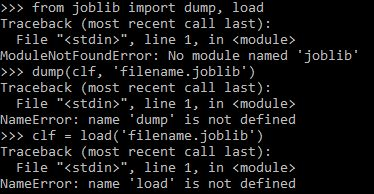
\includegraphics[width=0.75\textwidth]{figures/18.JPG}}\caption{Hasil Tampilan Error.}\end{figure}
\subsubsection{Tuliskan Kode Eror dan Jenis Erornya}
\begin{itemize}
\item \begin{verbatim}from joblib import dump, load\end{verbatim} (Kode baris pertama)
\subitem \begin{verbatim}
Traceback(most recent call last):
 File "<stdin>", line 1, in<module>
ModuleNotFoundError: No module named 'joblib'
\end{verbatim} (Errornya)
\item \begin{verbatim}dump(clf, 'filename.joblib')\end{verbatim} (Kode baris kedua)
\subitem \begin{verbatim}
Traceback(most recent call last):
 File "<stdin>", line 1, in<module>
NameError: name 'dump' is not defined
\end{verbatim} (Errornya)
\item \begin{verbatim}clf = load('filename.joblib')\end{verbatim} (Kode baris ketiga)
\subitem \begin{verbatim}
Traceback(most recent call last):
 File "<stdin>", line 1, in<module>
NameError: name 'load' is not defined
\end{verbatim} (Errornya)
\end{itemize}

\subsubsection{Solusi Pemecahan Masalah Error}
\begin{enumerate}
\item Pada masalah error sebelumnya itu dikarenakan kita belum mempunyai packaged joblib. Jadi solusinya yaitu dengan cara menginstall terlebih dahulu packaged joblibnya setelah itu baru perintah tersebut dapat dijalankan

\begin{figure}[ht]\centerline{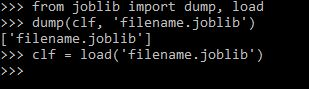
\includegraphics[width=0.75\textwidth]{figures/32.JPG}}\caption{Hasil Tampilan Uji coba perintah joblib.}\end{figure}
\end{enumerate}

>>>>>>> 78cdb6514db9716f252ef2024a7df6097aace611



